\lettrine[lines=2,lraise=0]{O}h I didn't find a goddess that looked the same, although she certainly is gorgeous. She didn't have an underground palace that I've read. Perhaps she has a sexy smirk but what mattered was Lilith is a wife and mother. A feminist. Confident and strong. Nurturing but viscous and powerful when defending her family.

She also is not in silk and heels, and prefers combat fatigues, or ivy league clothing, or whatever is advantageous. Get things done the hard way, then if she needs to use her sexuality it will be like a trump card. Her nature makes it so. Lilith on the other hand is always naked or in see through silky garments. That is one difference between them and that's just fine. 

Susan and Lilith both are of course, typical anti-heroes, shamelessly brutal and viscious. I would say that neither of their stories revolve around men. They are their own selves with their own goals and responsibilities.

	
She has many titles. Queen of Night and Darkness, Queen of Vampires, Lady Lilith, The Dark Mother. She likes different kinds of flowers including roses. She likes sandalwood incense. Her favourite fruit is pomegranate, and she loves chocolate.

At least one occultist who, as they say, worked with her, calls her an amazing lady.


\begin{wrapfigure}{R}{0.4\textwidth}
	\centering
	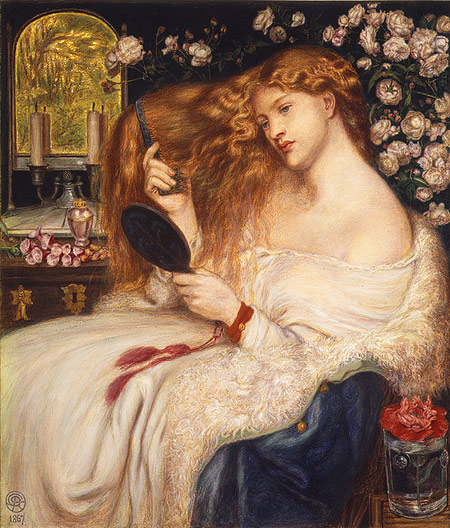
\includegraphics[width=0.40\textwidth]{Images/Rossetti_lady_lilith_1867}
	\\ {\small Rosetti 1867, Lady Lilith.}
\end{wrapfigure}


She, like Susan, was human once. She was the first woman. You see, women did not actually come from Adams rib. At least not the first. Lilith and Adam were both created from the dust to be each others companion. Adam preferred for her to be obedient to him and she preferred to have an equal partner and when that didn't work out she left. God only knows where she went but along the way she met Sam\ae l and they have been inseparable ever since.

She is the worlds first polyamorous woman. Sam\ae l may be her primary so to speak but she has had many lovers. Unlike the accusations of her being a whore though she genuinely loves those she is with and is quite happy, her and Sam\ae l are still together so they are an example of a successful polyamorous relationship.

She is a fierce advocate of women's sexuality, she enjoys sex with both men and women(not physically I assume, she's a d\ae mon), so as a result is an LGBT advocate. I'm sure that she is a 3rd generation feminist. She protects pregnant women and children. She is a healer. Although she heals through the feminine current she heals both men and women, especially with self image.

She is drop dead gorgeous. Everyone who sees her sees her differently but the description I was given makes her sound like an irish sex god. Long wavy red hair, pale skin and red lips, deep emerald green eyes, perfect body. She either wears nothing or majestic see through clothing.

What I have said I have said. There is such a conflicting mess in the field of demonology. Lilith likely has a dozen names at least. Her three most popular are Lilith, Lamia and Lamashtu. Sure they could be different entities but Lamashtu for one was described as being the daughter of heaven. In the context given it meant that God created her from nothing, as opposed to coming from man or woman. That has to be Lilith. 

Why is Lilith often described as evil incarnate? Sexually liberated feminist women and LGBT people are discriminated against now, whether they were Gods or not how would people have treated them or spoken of them in 1000BC or even before? People are so quick to see monsters around them, if only they would spend that time looking for the monsters inside themselves.